\subsection{Incrementally maintain the output of general linear algebra programs}
In data analytics, linear algebra programs are quite ubiquitous. Typical use of linear algebra programs includes computing the model parameters or labeling the samples as Section \ref{sec: maintain_model_para} and Section \ref{sec: maintain_classification} focus on, which usually involve updates to the input matrix data. To effectively propagate the updates through linear algebra programs to the output, there are some efforts which materialize the output of the linear algebra programs as views and incrementally maintain the view content. One example is Linview \cite{nikolic2014linview}, which expresses the updates to the input as {\em delta expression} and targets at propagating such {\em delta expression} through the iterative linear algebra programs with basic matrix operations, i.e. matrix addition, multiplication, subtraction, transpose and inverse, to update the result of the programs rather than re-evaluation from the scratch. In what follows, how the authors of \cite{nikolic2014linview} model the iterative linear algebra programs, represent and propagate {\em delta expressions} through the linear algebra program and deal with typical linear algebra programs are elaborated respectively.

\subsubsection{Model the iterative programs}\label{sec: iterative_model}
Iterative computation is very common in linear algebra programs, for which naive re-evaluation from the scratch in the case of data updates can incur high overhead. Under the assumption that the iterative programs end after a fixed number of iteration steps (even after updates), Linview models iterative computation in three different ways, i.e. {\em Linear model}, {\em Exponential model} and {\em Skip model}.
% delta expression propagation through the program under three different iterative models.

\paragraph{Linear model} The first iterative model is {\em linear model}, which simply updates the result at $k_{th}$ epoch based on the results at $(k-1)_{th}$ epoch. Given the input $A$, the output at epoch $k$, $T^{(k)}$ is computed as:

\[T^{(k)}=
\begin{cases}
f(A)& k=1\\
g(T^{(k-1)}, A) & k=2,3,\dots\\
\end{cases}
\]

where $f$ and $g$ represent the modified version of the original linear algebra programs that fit the linear model. $g(T^{(k-1)}, A)$ means that the value of $T^{(k)}$ depends on the value at the $(k-1)_{th}$ epoch and the input, i.e.  $T^{(k-1)}$ and $A$.

\paragraph{Exponential model} In the {\em exponential model}, the output at $k_{th}$ epoch depends on the result at $(k/2)_{th}$ epoch, which has larger leaps compared to {\em linear model}, i.e.:

\[
T^{(k)}=
\begin{cases}
f(A)& k=1\\
g(T^{(k/2)}, A) & k=2,4,8\dots\\
\end{cases}
\]

where $g(T^{(k/2)}, A)$ means that the value of $T^{k}$ is derived from the result at $k/2$ epoch and the input, i.e. $T^{(k/2)}$ and $A$.

\paragraph{Skip model} {\em Skip model} lies in between, in which the step between the computed iterations is adjustable. Given a skip size $s$, the result before $s_{th}$ epoch is computed by {\em exponential model} and then the result after $s_{th}$ epoch is computed every $s_{th}$ iteration. The {\em skip model} is thus represented as:

\[
T^{(k)}=
\begin{cases}
f(A)& k=1\\
g(T^{(k/2)}, A) & k=2,4,8\dots,s\\
h(T^{(k-s)}, T^{(s)}, A) & k=s, 2s,\dots
\end{cases}
\]

where $g(T^{(k/2)}, A)$ is the same as the one in {\em Exponential model} while $h(T^{(k-s)}, T^{(s)}, A)$ indicates that computing the result at $k_{th}$ epoch depends on the result at $(k-s)_{th}$ and $s_{th}$ epoch as well as the input, i.e. $T^{(k-s)}$, $T^{(s)}$ and $A$

\subsubsection{Incremental computation}
This subsection is centered around how Linview represent and propagate delta expression through the linear algebra programs, which starts by introducing the incremental updates over matrix manipulation primitives. Since matrix multiplications are frequently used in the linear algebra programs, it is assumed to have time complexity $O(n^{\gamma})$ ($2 < \gamma \leq 3$, varies for different algorithms)

\paragraph{Delta rules for basic matrix operations}
Given an $n \times n$ matrix $A$ and a function $f(*)$, small changes $\Delta A$ to $A$ leads to the changes of output of $f(A)$ as: $\Delta_A(f) = f(A+\Delta A) - f(A)$. By following the properties of basic matrix operations, such as matrix addition, matrix multiplication and matrix inverse, the delta rule is shown as follows:

\begin{center}
    \begin{minipage}{0.4\textwidth}
      \begin{itemize}
        \item $\Delta_A(f_1 f_2) = f_2\Delta_A(f_1) + f_1\Delta_A(f_2)$
        \item $\Delta_A(f_1 \pm f_2) = \Delta_A(f_1) \pm \Delta_A(f_2)$
        \item $\Delta_A(\lambda f) = \lambda \Delta_A(f)$
        \item $\Delta_A(f^{-1}) = f(A+\Delta A)^{-1}-f(A)^{-1}$
      \end{itemize}
    \end{minipage}
  \end{center}

Note that for most update rules shown above, the time complexity is $O(n^2)$ while in general case, the delta derivation for matrix inverse has the same overhead as reevaluation from the scratch, which is much more expensive than $O(n^2)$. However, under the assumption that $\Delta A$ only touches small portions of $A$, indicating that the rank of $\Delta A$, $k$ should be much smaller than that of $A$, i.e. $k \ll n$, $\Delta A$ can be decomposed into additions and multiplications of vectors and thus much cheaper for computation. The decomposed form of $\Delta A$ is called {\em factored form}. For example, given a rank-1 $\Delta A$ ($=\bar{u}\bar{v}^T$), by applying Sherman-Morrison formula \cite{press2007numerical}, $\Delta_A(f^{-1})$ can be written as:

\begin{equation}\label{eq: matrix_inverse}
\Delta_A(f^{-1}) = -\frac{f(A)^{-1}\bar{u}\bar{v}^Tf(A)^{-1}}{1+\bar{v}^Tf(A)^{-1}\bar{u}}
\end{equation}

\paragraph{Delta representation}
The overhead of the incremental updates also relies on how to represent the delta. It has turned out that naive representations won't help even for very simple program with very minor changes. 

\begin{example}\label{eg: incremental_naive_update}
For example, consider the following program to compute $A^8$ for an $n\times n$ matrix $A$:

\begin{center}
    $B:= AA$\\
    $C:= BB$\\
    $D:= CC$
\end{center}

Given a small change $\Delta A$, such as an update to the entry $A_{i,j}$, $\Delta A_{i,j}$, the time complexity of which is $O(1)$, by applying the delta rules for matrix multiplication mentioned above, $\Delta B$, $\Delta C$ and $\Delta D$ are represented as:

\begin{equation}\label{eq: delta_b}
    \Delta B = (\Delta A) A + A (\Delta A) + (\Delta A) (\Delta A)
\end{equation}
\begin{equation}\label{eq: delta_c}
    \Delta C = (\Delta B) B + B (\Delta B) + (\Delta B) (\Delta B)
\end{equation}
\begin{equation}\label{eq: delta_d}
    \Delta D = (\Delta C) C + C (\Delta C) + (\Delta C) (\Delta C)
\end{equation}
    


Computing $\Delta B$ only requires $O(n)$ operations since $(\Delta A) A$ and $A (\Delta A)$ only need to scale the $i_{th}$ row and $j_{th}$ column of $A$ by $\Delta A_{i,j}$ respectively, which takes $O(n)$ time while $(\Delta A) (\Delta A)$ only incurs $O(1)$ overhead. In the end, compared to original $B$, the changes caused by $\Delta B$ appear in the $i_{th}$ row and $j_{th}$ column of $B$.

Similarly, we can derive that $\Delta C$ requires $O(n^2)$ operations, which ends up with the propagation of the initial updates to the entire $C$. The effect of update propagation is shown in Figure \ref{fig:update_propagete}.

\begin{figure}
    \centering
    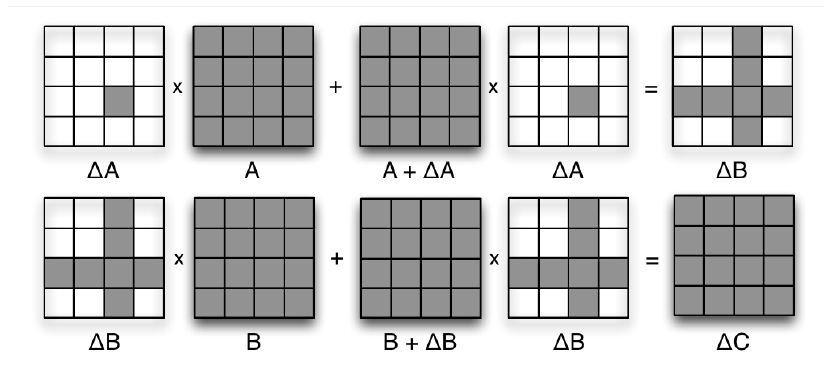
\includegraphics[width=10cm, height=4cm]{Figures/update_propagation.png}
    \caption{The effect of updates propagate}
    \label{fig:update_propagete}
\end{figure}

Then computing $\Delta D$ involves at least two full $O(n^{\gamma})$ matrix multiplications, which is obviously more expensive than recomputing $\Delta D$ from the scratch. \qed
\end{example}


To deal with such unexpected effect, as Example \ref{eg: incremental_naive_update} indicates, the updates $\Delta A$ is only a change to a single entry $A_{i,j}$, which is a rank-1 update and can be represented as $\Delta A = \bar{u}\bar{v}^T$ where $\bar{u}$ and $\bar{v}$ are both column vectors. Then by replacing $\Delta A$ in Equation \ref{eq: delta_b} with $\bar{u}\bar{v}^T$, $\Delta B$ is rewritten as:
\begin{equation}\label{eq: update_b_product}
\Delta B = \bar{u}(\bar{v}^TA) + (A\bar{u})\bar{v}^T + (\bar{u}\bar{v}^T\bar{u})\bar{v}^T=[\bar{u}, (A\bar{u}), (\bar{u}\bar{v}^T\bar{u})]
\begin{bmatrix}
    (\bar{v}^TA)  \\
    \bar{v}^T  \\
    \bar{v}^T   
\end{bmatrix}
=[\bar{u}_1, \bar{u}_2, \bar{u}_3]
\begin{bmatrix}
    \bar{v}^T_1  \\
    \bar{v}^T_2  \\
    \bar{v}^T_3  
\end{bmatrix}
\end{equation}

which is a sum of three outer products between vectors. The term $(\bar{v}^TA)$, $(A\bar{u})$ and $(\bar{u}\bar{v}^T\bar{u})$ can be all derived in $O(n^2)$ time while the vector $[\bar{u}, (A\bar{u}), (\bar{u}\bar{v}^T\bar{u})]$ and $[(A^T\bar{v}), \bar{v}, \bar{v}]$ are both $n \times 3$ matrices and thus computing $\Delta B$ in this way requires $O(3n^2)$ operations.

Although it is more expensive than naive updates for $\Delta B$ as shown in Example \ref{eg: incremental_naive_update}, in general, all the delta expressions can be expressed as a product of two $n \times k$ matrices where $k \ll n$, which only requires $O(kn^2)$ operations. For example, for $\Delta C$, since it is a sum of three products, i.e. $\Delta B B$, $B \Delta B$ and $\Delta B \Delta B$, and each of them can be expressed as a product of two $n \times 3$ matrices by plugging Equation \ref{eq: update_b_product} into Equation \ref{eq: delta_c}, $\Delta C$ can thus be expressed as a a product of two $n \times 9$ matrices:


\begin{equation}
\begin{split}
    \Delta C &= (\Delta B) B + B (\Delta B) + (\Delta B) (\Delta B) \\&=[\bar{u}_1, \bar{u}_2, \bar{u}_3]
\begin{bmatrix}
    \bar{v}^T_1B \\
    \bar{v}^T_2B \\
    \bar{v}^T_3B 
\end{bmatrix}+[B\bar{u}_1, B\bar{u}_2, B\bar{u}_3]
\begin{bmatrix}
    \bar{v}^T_1 \\
    \bar{v}^T_2 \\
    \bar{v}^T_3 
\end{bmatrix}\\
&+[\bar{u}_1, \bar{u}_2, \bar{u}_3]
\begin{bmatrix}
    \bar{v}^T_1  \\
    \bar{v}^T_2  \\
    \bar{v}^T_3  
\end{bmatrix}
[\bar{u}_1, \bar{u}_2, \bar{u}_3]
\begin{bmatrix}
    \bar{v}^T_1  \\
    \bar{v}^T_2  \\
    \bar{v}^T_3  
\end{bmatrix}\\
&=[\bar{u}_1, \bar{u}_2, \bar{u}_3, B\bar{u}_1, B\bar{u}_2, B\bar{u}_3, \bar{u}_1, \bar{u}_2, \bar{u}_3]\\
&\begin{bmatrix}
    \bar{v}^T_1B \\
    \bar{v}^T_2B \\
    \bar{v}^T_3B \\
    \bar{v}^T_1  \\
    \bar{v}^T_2  \\
    \bar{v}^T_3  \\
    \bar{v}^T_1(\bar{u}_1\bar{v}^T_1 + \bar{u}_2\bar{v}^T_2 + \bar{u}_3\bar{v}^T_3)\\
    \bar{v}^T_2(\bar{u}_1\bar{v}^T_1 + \bar{u}_2\bar{v}^T_2 + \bar{u}_3\bar{v}^T_3)
    \bar{v}^T_3(\bar{u}_1\bar{v}^T_1 + \bar{u}_2\bar{v}^T_2 + \bar{u}_3\bar{v}^T_3)
\end{bmatrix}
\end{split}
\end{equation}

which requires $O(9n^2)$ operations in total. Finally, by plugging the expression of $\Delta C$ above into Equation \ref{eq: delta_d}, computing $D$ only requires $O(27n^2)$ operations, which is far cheaper than re-evaluation from the scratch especially when $n$ is large.

Actually, $\Delta B$ can be further optimized as:
\begin{equation}\label{eq: update_b_product_opt}
\Delta B = \bar{u}(\bar{v}^TA) + (A\bar{u})\bar{v}^T + (\bar{u}\bar{v}^T\bar{u})\bar{v}^T=[\bar{u}, (A\bar{u}) + (\bar{u}\bar{v}^T\bar{u})]
\begin{bmatrix}
    (\bar{v}^TA)  \\
    \bar{v}^T 
\end{bmatrix}
=[\bar{u}_1', \bar{u}_2']
\begin{bmatrix}
    \bar{v}^T_1'  \\
    \bar{v}^T_2'  \\
\end{bmatrix}
\end{equation}

which is a product of two $n \times 2$ matrices. Consequently, $\Delta C$ and $\Delta D$ can be represented as a product of two $n \times 4$ matrices and two $n \times 8$ matrices respectively.

\paragraph{In the case of programs with multiple inputs}
Given the derivation rules above, Linview can also handle the case where the linear algebra programs have multiple inputs and each of them may involve updates. \eat{converts the linear algebra program into a set of trigger functions, which takes a set of input matrices and handle the updates of them sequentially. }For example, given a set of input matrices $D=\{A, B, \dots\}$ and an evaluation function $f(*)$ over that, then the overall effect of updates to $f(D)$ will be:

\begin{equation}\label{eq: updates_by_multi_vars}
\Delta_{D}(f(D)) = \Delta_{A}(f(D)) + \Delta_{D \setminus \{A\}}(f(D) + \Delta_{A}(f(D)))
\end{equation}


%  and Linview generates one trigger function for each of them, which is then used to monitor the change of the corresponding input matrix.

\subsubsection{Incremental analysis for typical programs}\label{sec: analysis_typical_programs}
The incremental update model above can fit some typical linear algebra programs, such as regression model, matrix powers and even more general forms, which are illustrated below.

\paragraph{Regression model}
Recall that in Section \ref{sec: pre}, for regression model, given an $m \times n$ matrix $X$ for predictor variables and an $m \times p$ matrix $Y$ for response variables, where there are $m$ data points, $n$ features and $p$ response variables in total, the coefficient $W^*$ is estimated as $W^* = (X^TX)^{-1}X^TY$.

In practice, the regression model is usually built in a dynamic environment where the incoming new data requires efficient incremental updates to $W^*$ instead of computing from the scratch every time, for which the performance bottleneck is to update the inverse operation $(X^TX)^{-1}$. We represent $X^TX$ as $Z$. So given a rank-1 update to $X$, i.e. $\Delta X = \bar{u}\bar{v}^T$, $\Delta Z$ can be expressed as:
\begin{equation}\label{eq: regression_factor}
    \Delta Z = [\bar{v}\ \ (X^T\bar{u} + \bar{v}\bar{u}^T\bar{u})]\begin{bmatrix}
    \bar{u}^T X  \\
    \bar{v}^T  
\end{bmatrix}\\
=[\bar{p}_1\ \bar{p}_2]\begin{bmatrix}
    \bar{q}^T_1  \\
    \bar{q}^T_2  
\end{bmatrix}=\bar{p}_1\bar{q}_1^T + \bar{p}_2\bar{q}_2^T
\end{equation}

The time complexity of Equation \ref{eq: regression_factor} is $O(mn)$ due to the computation of $X^T\bar{u}$, $\bar{v}\bar{u}^T\bar{u}$ and $\bar{u}^TX$, which ends up with a product of two $n\times 2$ matrices and thus a rank-2 update to $Z$. We can further represent $\Delta Z$ as the sum of $\Delta Z_1$ and $\Delta Z_1$ where $\Delta Z_1 = \bar{p}_1\bar{q}_1^T$ and $\Delta Z_2 = \bar{p}_2\bar{q}_2^T$ such that $\Delta Z_1$ and $\Delta Z_2$ are both rank-1 matrix. Considering the fact that both $X$ and $\Delta X$ are $m \times n$ matrices and thus $\bar{u}$ and $\bar{v}$ are $m \times 1$ and $n \times 1$ vector respectively, $\bar{p}_1$ and $\bar{q}_2$ should be both $n \times 1$ vectors. Besides, the computation result of $X^T\bar{u}$ and $\bar{v}\bar{u}^T\bar{u}$ are both $n \times 1$ vector and thus $\bar{p}_2$ (sum of $X^T\bar{u}$ and $\bar{v}\bar{u}^T\bar{u}$) should be also $n \times 1$ vector. Similarly, $\bar{q_1}^T$ is also $n \times 1$ vector.

By following Equation \ref{eq: matrix_inverse} and Equation \ref{eq: updates_by_multi_vars}, the update rules for $J = (X^TX)^{-1} = Z^{-1}$ with respect to $\Delta Z_1$ and $\Delta Z_2$ will be:

\begin{center}
\begin{equation}
\begin{split}
    \Delta_{Z_1}(J)& = -\frac{J\bar{p}_1\bar{q}_1^TJ}{1 + \bar{q}_1^TJ\bar{p}_1}\\
    \Delta_{Z_2}(J)& = -\frac{(J+\Delta_{Z_1}(J))\bar{p}_2\bar{q}_2^T(J+\Delta_{Z_1}(J))}{1 + \bar{q}_2^T(J+\Delta_{Z_1}(J))\bar{p}_2}
\end{split}   
\end{equation}
\end{center}

which computes the rank-1 update $\Delta Z_1$ to $J$ and then accumulate the effect when propagating $\Delta Z_2$ for $J$. $\Delta_{Z_1}(J)$ and $\Delta_{Z_2}(J)$ can be further written as:

\begin{equation}
\begin{split}
\Delta_{Z_1}(J) = \bar{r}_1\bar{s}_1^T\\    
\Delta_{Z_2}(J) = \bar{r}_2\bar{s}_2^T
\end{split}
\end{equation}

where $\bar{r}_1 = J\bar{p}_1$, $\bar{r}_2 = (J+\Delta_{Z_1}(J))\bar{p}_2$ while $\bar{s}_1$ and $\bar{s}_2$ are the rest of the subexpressions of $\Delta_{Z_1}(J)$ and $\Delta_{Z_2}(J)$ respectively. So the overall updates to $J$ is $\Delta J = \bar{r}_1\bar{s}_1^T + \bar{r}_2\bar{s}_2^T$, which is a rank-2 update.
Since $\bar{p}_i$ and $\bar{q}_i$ ($i=1,2$) are column vector of length $n$ and $Z$ and $J$ are $n \times n$ matrices, the computation of $\bar{r}_1 =J\bar{p}_1$ thus need $O(n^2)$ operations, which is the same for $\bar{s}_1$, $\bar{s}_2$ and $\bar{r}_2$. So the overall cost to update $J$ is thus $O(n^2 + mn)$, which is far less than the cost of recomputing from the scratch, i.e. $O(n^3 + mn)$.

In terms of the update for $W^*$ (denoted by $\Delta W$), given the update to the input $X$, i.e. $\Delta X=\bar{u}\bar{v}^T$, $\Delta W$ can be thus written as:

\begin{equation}
\begin{split}
    \Delta W &= \Delta ((X^TX)^{-1}X^TY) = \Delta(JX^TY)= \Delta JX^TY + J\Delta X^TY + \Delta J\Delta X^TY\\
    &= (\bar{r}_1\bar{s}_1^T + \bar{r}_2\bar{s}_2^T)X^TY + J\bar{v}\bar{u}^TY + (\bar{r}_1\bar{s}_1^T + \bar{r}_2\bar{s}_2^T)\bar{v}\bar{u}^TY
\end{split}
\end{equation}

while requires $O(n^2 + mp + np + mn)$ operations in total while re-evaluation incurs $O(mnp + n^2min(m,p))$ operations.

\paragraph{Matrix powers}
The goal of matrix powers is to compute $A^k$ for an input matrix $A$ with a given exponent $k$, which plays an important role in many data analysis tasks. Matrix powers can be computed iteratively, for which the three iterative models proposed in Section \ref{sec: iterative_model} are applicable and the trade-offs between the three models are explored under re-evaluation strategy or incremental update strategy. The results are presented in Table \ref{tab:time_space_complexity_matrix_power} under the assumption $k \ll n$.

% \begin{figure}
%     \centering
%     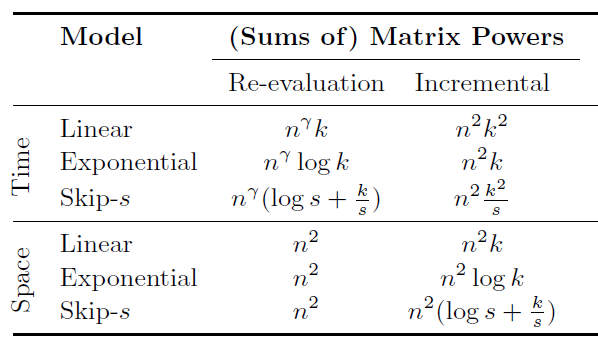
\includegraphics[width=8cm, height=4.5cm]{Figures/time_space_complexity_matrix_powers.png}
%     \caption{The time and space trade-offs for matrix power}
%     \label{fig:time_space_complexity_matrix_power}
% \end{figure}
\begin{table}[h]
    \centering
    \begin{tabular}{|c|c|c|c|}\hline
        &\multirow{2}{*}{Model} & \multicolumn{2}{|c|}{(Sum of) Matrix Powers}  \\\hhline{~~--}
        &&Re-evaluation & Incremental\\ \hline
    \multirow{3}{*}{Time}&Linear & $n^{\gamma}k$ & $n^2k^2$\\\hhline{~---}
    &Exponential & $n^{\gamma}log k$ & $n^2k$\\\hhline{~---}
    &Skip-s & $n^{\gamma}(logs+\frac{k}{s})$ & $n^2\frac{k^2}{s}$\\\hline
    \multirow{3}{*}{Space}&Linear & $n^2$ & $n^2k$\\\hhline{~---}
    &Exponential & $n^2$ & $n^2log k$\\\hhline{~---}
    &Skip-s & $n^2$ & $n^2(logs+\frac{k}{s})$\\\hline
    \end{tabular}
    \caption{The time and space trade-offs for (sum of) matrix power}
    \label{tab:time_space_complexity_matrix_power}
\end{table}

For re-evaluation strategy, it would require $O(n^{\gamma})$ operations for matrix multiplication at every iteration and thus the total time complexity depends on the number of iterations. Thus Exponential model outperforms the other models since it has largest leap between iterations. But all of the models have the same space complexity, i.e. $O(n^2)$.

For incremental update strategy, the computation time at each iteration should be $O(rn^2)$ where $r$ is the rank of the input delta expression, which may vary at different epochs. For example, under Exponential model, as Example \ref{eg: incremental_naive_update} shows, $r$ doubles after each epoch. Since there are $logk$ iterations in total, the overall time complexity would be $O(n^2(1+2+2^2+\dots+2^{logk})) = O(n^2k)$. In contrast, $r$ increases linearly under linear model, which leads to quadratic running time in the end with respect to the iteration number $k$, i.e. $O(n^2k^2)$. Under skip-s model, since the value of $T^{(k)}$ needs $T^{(s)}$ and $T^{(k-s)}$, which are products of two $n\times s$ matrices and two $n\times (k-s)$ matrices respectively. When $\Delta T^{(s)}$ and $\Delta T^{(k-s)}$ are given, $\Delta T^{(k)} = \Delta T^{(s)}T^{(k-s)} + \Delta T^{(k-s)}T^{(s)}$, which requires $O(n^2k)$ operations in total. Suppose the time complexity to compute $\Delta T^{(k)}$ is $f(k)$, since $(k-s)_{th}$ epoch may not necessarily be prior to $s_{th}$ epoch, the result at which also needs to be computed by referencing the result at $(k-2s)_{th}$ epoch and the $s_{th}$ epoch, i.e. $\Delta T^{(k-s)} = \Delta T^{(s)}T^{(k-2s)} + \Delta T^{(k-s)}T^{(s)}$, then $f(k) = f(k-s) + O(n^2k)$. By induction, $f(k) = O(n^2\frac{k^2}{s})$.

Similar to {\em matrix power}, the sum of matrix power problem, which aims at computing $S^{(k)} = I + A + A^2 + \dots + A^k$ given input $A$ and maximum exponent $k$ where $I$ is the identity matrix, have the almost the same computation process and thus have the same time complexity as shown in Table \ref{tab:time_space_complexity_matrix_power}. 

\paragraph{General form} The authors also consider a general iterative matrix computation programs based on matrix powers, i.e. $T^{(i+1)} = AT^{(i)} + B$ where $A$ is the input matrix with dimension $n \times n$, $B$ is a constant matrix with dimension $n \times p$ and the result $T^{(i)}$ is iteratively computed which has dimension $n \times p$. Such general form appears in many applications such as PageRank and power iteration method for eigenvalue computation. 

Note that $T^{(i+1)} = AT^{(i)} + B$ can be unrolled as the following form by referencing the results at iteration $i$ and previous iterations, i.e. $T^{(i+k)} = A^kT^{(i)} + (A^{k-1} + A^{k-2} + \dots + A + I) B$, in which how to efficiently incrementally compute $P^{(k)} = A^k$ and $S^{(k)} = (A^{k-1} + A^{k-2} + \dots + A + I)$ has been discussed before and thus both $P^{(k)}$ and $S^{(k)}$ are materialized and maintained along with $T^{(k)}$. Given those notations, the derivation rules for $T^{(i+1)} = AT^{(i)} + B$ under the three iterative models from Section \ref{sec: iterative_model} are shown in Table \ref{tab:derivation_rule}.


% \begin{table}[t]
%     \centering
%     \begin{tabular}{|c|c|}\hline
%         Model & Derivation rule \\ \hline
%         Linear & $T^{(k)}=
% \begin{cases}
% A& k=1\\
% AT^{(k-1)} & k=2,3,4\dots
% \end{cases}$\\ \hline
%         Exponential & $T^{(k)}=
% \begin{cases}
% A& k=1\\
% T^{(k/2)}T^{(k/2)} & k=2,4,8\dots,s\\
% \end{cases}$\\ \hline
%         Skip-s &$T^{(k)}=
% \begin{cases}
% A& k=1\\
% T^{(k/2)}T^{(k/2)} & k=2,4,8\dots,s\\
% T^{(s)}T^{(k-s)} & k = 2s, 3s, \dots, k
% \end{cases}$\\ \hline
%     \end{tabular}
%     \caption{Derivation rules for $T^{(k)} = A^{k}$ under three iterative models}
%     \label{tab:derivation_rule}
% \end{table}






\begin{table}[t]
    \centering
    \begin{tabular}{|c|c|}\hline
        Model & Derivation rule \\ \hline
        Linear & $T^{(k)}=
\begin{cases}
AT^{(0)} + B& k=1\\
AT^{(k-1)} + B & k=2,3,4\dots
\end{cases}$\\ \hline
        Exponential & $T^{(k)}=
\begin{cases}
AT^{(0)} + B& k=1\\
P^{(k/2)}T^{(k/2)} + S^{(k/2)}B & k=2,4,8\dots,s\\
\end{cases}$\\ \hline
        Skip-s &$T^{(k)}=
\begin{cases}
AT^{(0)} + B& k=1\\
P^{(k/2)}T^{(k/2)} + S^{(k/2)}B & k=2,4,8\dots,s\\
P^{(s)}T^{(k-s)} + S^{(s)}B & k = 2s, 3s, \dots
\end{cases}$\\ \hline
    \end{tabular}
    \caption{Derivation rules for $T^{(i+1)} = AT^{(i)} + B$ under three iterative models}
    \label{tab:derivation_rule}
\end{table}

Then given an update $\Delta A$ against the input matrix $A$, the cost analysis under different iterative models and update strategies is provided below.

In terms of re-evaluation strategy, the results of $T^{(i)}$, $P^{(i)}$ and $S^{(i)}$ are only materialized for current iteration. For linear model, computing $AT^{(i)}$ is the performance bottleneck, which requires one multiplication of two $n \times 1$ vectors for every entry at the result $AT^{(i)}$ and $O(np)$ such multiplications in total. So the time complexity to compute $AT^{(i)}$ at each epoch is $O(pn^2)$, which incurs time complexity $O(kpn^2)$ for $k$ iterations. For exponential model and skip-s model, maintaining $P^{(i)}$ and $S^{(i)}$ would incur time complexity $O(n^{\gamma})$ for every iterations, which is essential for $logk$ and $logs + \frac{k}{s}$ iterations respectively. Besides the cost of maintaining the auxiliary matrices $P^{(i)}$ and $S^{(i)}$, it still needs $O(pn^2)$ time to compute $P^{(s)}T^{(i-s)}$ or $P^{(i/2)}T^{(i/2)}$ at each iteration. Since the number of iterations for exponential model and skip-s model is $logk$ and $logs + \frac{k}{s}$ respectively, the overall time complexity for the two models will be $O(n^{\gamma} + pn^2)logk$ and $O(n^{\gamma}logs + pn^2(logs+ \frac{k}{s}))$.

For incremental strategy, the time complexity to incrementally update $P^{(s)}$ and $S^{(s)}$ is still $O(rn^2)$ for each iteration as discussed before where $r$ is the rank of the factored forms of $P^{(s)}$ and $S^{(s)}$. To derive $T^{(k)}$, the update rule $P^{(i/2)}T^{(i/2)} + S^{(i/2)}B$ or $P^{(s)}T^{(i-s)} + S^{(s)}B$ is used, which requires extra $O(np)$ time to compute the factored form for $T^{(i)}$. So the overall time complexity for each iteration will be $O(n^2 + np)$. By following similar analysis for {\em matrix powers}, the time complexity and space complexity for the three different iterative models is presented in Table \ref{tab:time_space_complexity_general_form}.

But notice that for some extreme case, such as $p=1$, incremental update strategy has worse performance than re-evaluation strategy, which is due to the unnecessary factor form representations for $T^{(i)}$ (a vector in this case). To solve this problem, a combination of the re-evaluation strategy and incremental updates strategy called Hybrid strategy is proposed, which simply represent delta expression for $T^{(i)}$ as a single matrix instead of two factored vectors and still represent the auxiliary matrix $P^{(i)}$ and $S^{(i)}$ in factored form. So for exponential model and skip-s model, they require $rn^2$ operations to update $P^{(i)}$ and $S^{(i)}$ for each iteration where $r$ is the rank of them, which incurs the same overhead as the incremental updates for matrix powers while the time complexity to compute $T^{(k)}$ is $O(pn^2)$ when $P^{(i)}$ and $S^{(i)}$ are given, which has the same time complexity as re-evaluation strategy. By summing up the time complexity from the two parts, the overall time complexity is presented in Table \ref{tab:time_space_complexity_general_form}. Since both $P^{(i)}$ and $S^{(i)}$ for hybrid strategy are materialized in the same form as incremental update strategy for every iteration, it thus shares the same space complexity as incremental update strategy.


% \begin{figure}
%     \centering
%     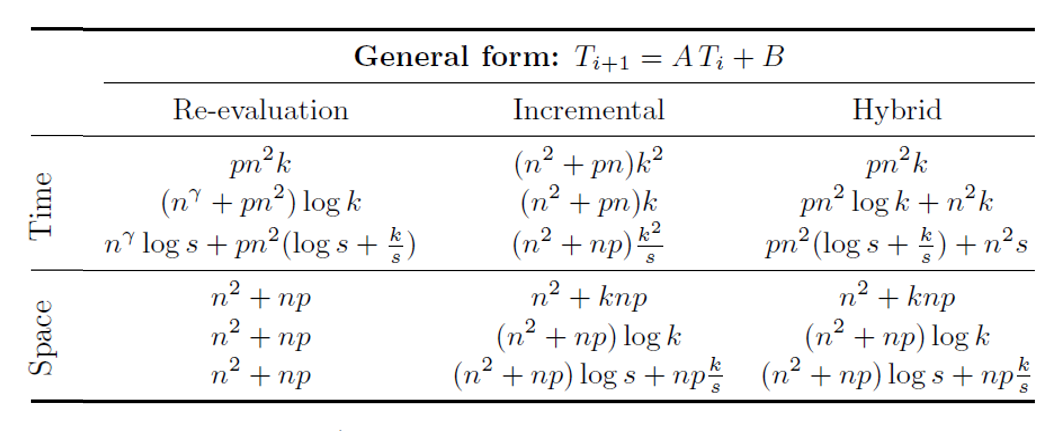
\includegraphics[width=12cm, height=4.5cm]{Figures/time_space_complexity_general_form.png}
%     \caption{The time and space trade-offs for general forms}
%     \label{fig:time_space_complexity_general_form}
% \end{figure}

\begin{table}[h]
    \centering
    \begin{tabular}{|c|c|c|c|c|}\hline
        &\multicolumn{4}{|c|}{$T^{(i+1)} = AT^{(i)} + B$}  \\\hhline{~----}
        &Model&Re-evaluation & Incremental&Hybrid\\ \hline
    \multirow{3}{*}{Time}&Linear & $pn^2k$ & $(n^2+pn)k^2$&$pn^2k$\\\hhline{~----}
    &Exponential & $(n^{\gamma}+pn^2)logk$ & $(n^2+pn)k$&$pn^2logk+n^2k$\\\hhline{~----}
    &Skip-s & $n^{\gamma}logs+pn^2(logs +  \frac{k}{s})$ & $(n^2+pn)\frac{k^2}{s}$&$pn^2(logs + \frac{k}{s}) + n^2s$\\\hline
    \multirow{3}{*}{Space}&Linear & $n^2 + np$ & $n^2+knp$&$n^2 + knp$\\\hhline{~----}
    &Exponential & $n^2 + np$ & $(n^2 + np)logk$& $(n^2 + np)logk$\\\hhline{~----}
    &Skip-s & $n^2 + np$ & $(n^2+np)(logs+np\frac{k}{s})$&$(n^2+np)(logs+np\frac{k}{s})$\\\hline
    \end{tabular}
    \caption{The time and space trade-offs for general forms}
    \label{tab:time_space_complexity_general_form}
\end{table}

\subsubsection{Experimental results}
To evaluate the performance of Linview, the authors run typical linear algebra programs mentioned in Section \ref{sec: analysis_typical_programs} over Spark and Octave, taking dense random matrices of dimension up to (100k $\times$ 100k) as input. Throughout those experiments, re-evaluation, incremental evaluation and hybrid computation are compared against each other under all the three iterative models, i.e. Linear model, Exponential model and Skip-s model if iterative computation exists. The prefixes ``Reeval'', ``Incr'', and ``Hybrid'' are used to denote traditional re-evaluation, incremental processing, and hybrid computation, respectively while the suffixes ``Lin'', ``Exp'', and ``Skip-s'' represent the Linear, Exponential, and Skip-s models, respectively.

\begin{figure}
    \centering
    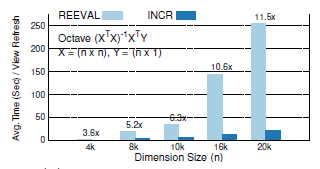
\includegraphics[height = 0.25\textwidth, width=0.5\textwidth]{Figures/linview_regression_exp.png}
    \caption{Time performance for linear regression in Linview}
    \label{fig:linview_linear_regression}
\end{figure}


The experimental results for linear regression is presented in Figure \ref{fig:linview_linear_regression}. It indicates that as the dimension of the matrix $X$ increases, incremental evaluation can achieve more speed-ups than re-evaluation, which is consistent with the complexity analysis in Section \ref{sec: analysis_typical_programs}.

For Matrix powers computation, with the fixed dimension ($n$) and iteration number $k$ for the input matrix $A$, the speed-up of incremental evaluation can be over 10x compared to reevaluation under all the iterative models, which is shown in Figure \ref{fig:linview_matrix_powers}. As Figure \ref{fig:linview_matrix_powers2} indicates, with the increase of the dimension of the input matrix, the performance gap between incremental evaluation and re-evaluation becomes larger. Note that in Figure \ref{fig:linview_matrix_powers2}, in the case of Spark backend, the running time is over one hour when the dimension $n$ is larger than 50k and thus not shown in the figure. SImilarly, orders of magnitude speed-ups are achieved with varied iteration number $k$ (see Figure \ref{fig:linview_matrix_powers3}).

\begin{figure}[h]
\captionsetup[subfigure]{width=1\textwidth}
     \centering
    \begin{subfigure}{0.3\textwidth}
        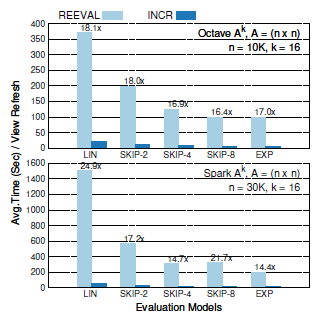
\includegraphics[height = 1.5\textwidth, width=1.2\textwidth]{Figures/linview_matrix_power_exp.png}
        \caption{}
        \label{fig:linview_matrix_powers}
    \end{subfigure}
    \hfill
    % \hspace{1.5cm}
    \begin{subfigure}{0.3\textwidth}
        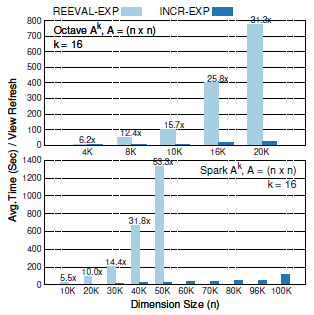
\includegraphics[height = 1.5\textwidth, width=1.2\textwidth]{Figures/linview_matrix_power_exp2.png}
    \caption{}
    \label{fig:linview_matrix_powers2}
    \end{subfigure}
    \hfill
    \begin{subfigure}{0.3\textwidth}
        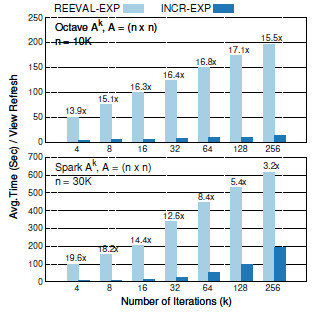
\includegraphics[height = 1.5\textwidth, width=1.2\textwidth]{Figures/linview_matrix_power_exp3.png}
    \caption{}
    \label{fig:linview_matrix_powers3}
    \end{subfigure}
    \caption{Time performance for Matrix powers in Linview}
\end{figure}

For the general form $T^{(i+1)} = AT^{(i)} + B$, as Figure \ref{fig:linview_general1} shows, with the fixed iterative models, such as linear model, hybrid computation strategy outperforms both re-evaluation and incremental evaluation in the case that $T$ has more row number than column number (i.e. $p \ll n$), which, however, incurs much more overhead than incremental evaluation in the case of large $p$ value. So it matches the time complexity analysis in Section \ref{sec: analysis_typical_programs}. The experimental results do not significantly depend on the specific iterative model, which is highlighted in Figure \ref{fig:linview_general2}.




% \begin{figure}
%     \centering
%     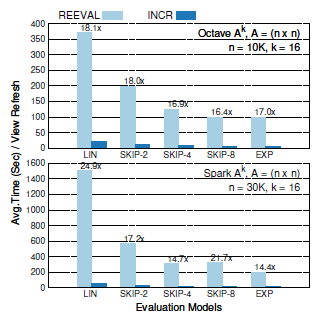
\includegraphics[height = 0.5\textwidth, width=0.5\textwidth]{Figures/linview_matrix_power_exp.png}
%     \caption{Time performance for Matrix powers in Linview}
%     \label{fig:linview_matrix_powers}
% \end{figure}

\begin{figure}
\captionsetup[subfigure]{width=1\textwidth}
     \centering
    \begin{subfigure}{0.35\textwidth}
        {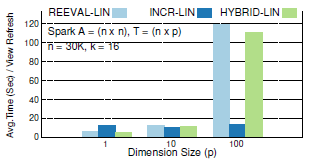
\includegraphics[height = 0.8\textwidth, width=1.2\textwidth]{Figures/linview_general_exp2.png}}
        \caption{}
        \label{fig:linview_general1}
    \end{subfigure}
    % \hfill
    \hspace{1.5cm}
    \begin{subfigure}{0.35\textwidth}
        {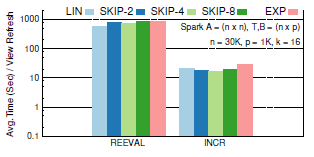
\includegraphics[height = 0.8\textwidth, width=1.2\textwidth]{Figures/linview_general_exp1.png}}
        % \caption{$t_{total}$ with varied $N_v$}
        \caption{}
        \label{fig:linview_general2}
    \end{subfigure}
    \caption{Time performance for general form $T^{(i+1)} = AT^{(i)} + B$ in Linview}
\end{figure}

% \begin{table}[h]
%     \centering
%     \begin{tabular}{|c|c|c|c|}\hline
%         &\multicolumn{3}{|c|}{$T^{(i+1)} = AT^{(i)} + B$}  \\\hhline{~---}
%         &Model&Re-evaluation & Incremental\\ \hline
%     \multirow{3}{*}{Time}&Linear & $pn^2k$ & $(n^2+pn)k^2$\\\hhline{~---}
%     &Exponential & $(n^{\gamma}+pn^2)logk$ & $(n^2+pn)k$\\\hhline{~---}
%     &Skip-s & $n^{\gamma}logs+pn^2(logs +  \frac{k}{s})$ & $(n^2+pn)\frac{k^2}{s}$\\\hline
%     \multirow{3}{*}{Space}&Linear & $n^2 + np$ & $n^2+knp$\\\hhline{~---}
%     &Exponential & $n^2 + np$ & $(n^2 + np)logk$\\\hhline{~---}
%     &Skip-s & $n^2 + np$ & $(n^2+np)(logs+np\frac{k}{s})$\\\hline
%     \end{tabular}
%     \caption{The time and space trade-offs for general forms}
%     \label{tab:time_space_complexity_general_form}
% \end{table}


\subsection{Discussions}
In this section, some recent work on incrementally updating views in the context of data analysis tasks is summarized, where the views can be model parameters \cite{deshpande2006mauvedb, gupta2015processing}, classification results \cite{koc2011incrementally} and the output of general linear algebra programs \cite{nikolic2014linview}. In this subsection, we explore other work related to this topic and discuss about potential drawbacks and limit of the works presented in this section.

\paragraph{Relationship to incremental view maintenance} 
Incrementally maintaining materialized views is a well-studied topic in database domain. For example, in relational database domain, \cite{gupta1993maintaining} studied how to incrementally maintain views for non-recursive views (possibly with negation and aggregation) when insertion or deletion happens in the underlying base relations, \cite{dong2000incremental} solves the same problem for recursive views and \cite{green2007update} deals with deletion propagation from the base relation tuples to the view instances by applying provenance semiring \cite{green2007provenance} in the context of update exchanges. Some efforts are also put on this problem in the context of semistructed database or graph database, e.g. \cite{liefke2000view} and \cite{abiteboul1998incremental}. As mentioned before, the papers introduced in this section share the same spirit with the incremental view maintenance efforts for traditional databases, which consider the model parameters, model prediction results or the linear algebra program output as ``views'' for incremental maintenance.

\paragraph{Relationship to online learning} Online learning is a technique that receives training data sequentially and updates the model based on the difference between the predication made by the current model and real label at each epoch to minimize some loss function \cite{DBLP:journals/corr/abs-1802-02871}. Incrementally updating model parameters discussed in Section \ref{sec: maintain_model_para} is similar to online learning problem but still differs in some aspects. First, the incremental updates over machine learning models should reflect the effect of both the addition and the removal of data points, which can be partially supported by some machine learning models. But there is no removal of data in online learning applications. Plus, unlike online learning, incremental updates over model parameters do not depend on the prediction correctness on new data. 

\paragraph{Relationship to data provenance} Data provenance identifies where a piece of data came from and the process by which it arrived in the database \cite{buneman2001and}.  It has been used to track the dependencies between inputs and outputs, detect errors in complex workloads, and provide explanations for debugging purposes. Various formulations of provenance have been studied, such as \textit{why- and where-provenance} \cite{buneman2001and}, \textit{why-not-provenance} \cite{chapman2009not}, and the \textit{provenance semirings} framework %(how-provenance) 
for conjunctive queries \cite{green2007provenance}, aggregate queries \cite{amsterdamer2011provenance} and queries with negation \cite{xu2018provenance}.  This framework has been used to implement several practical provenance-enabled database systems, such as ORCHESTRA \cite{ives2008orchestra} and GProM \cite{arab2018gprom}. Note that provenance has been applied for the purpose of view maintenance in ORCHESTRA \cite{ives2008orchestra}, particularly for reflecting the effect of deletion of base relation tuples to the view content. Considering the fact that in \cite{deshpande2006mauvedb} and \cite{gupta2015processing}, only a small portion of models, i.e. linear regression and Naive Bayes, can remove the effect of parts of the training data for a existing linear regression or Naive Bayes model and thus update the model in real time, which is similar to deletion propagation characteristic of data provenance. It is worth trying to apply data provenance to support model updates in the case of removal of partial training data for other machine learning models, such as logistic regression, K-means and SVM.



\paragraph{Relationship to interpretable machine learning} In machine learning community, one of the biggest concern is to interpret the behaviors of the machine learning models, which, however, are usually considered as ``black box'' due to their internal complexity. The interpretability of machine learning models can be divided into four categories, including {\em model explanation}, {\em outcome explanation}, {\em model inspection} and {\em transparent box design problem} according to a survey paper \cite{guidotti2018survey}. The incremental updates to the linear algebra program introduced in \cite{nikolic2014linview} is closely related to {\em model inspection} problem. It targets at measuring the effect of small variation of the test data to the accuracy in the test phase. So the model derived from the training phase is regarded as a program with matrix operations and thus the small changes of input can be propagated through programs in the same fashion as \cite{nikolic2014linview}. However, as highlighted later, \cite{nikolic2014linview} is unable to handle the non-linear operators which frequently appear in the machine learning algorithms. So it will not be trivial to apply \cite{nikolic2014linview} to {\em model inspection} problem. There are also increasing interests in understanding the black-box model by evaluating the ``influence'' of certain training data point $d$ for a machine learning \cite{koh2017understanding}, which is usually achieved by comparing the original model and the model constructed without including $d$ in the training dataset. So to efficiently update the model parameters by removing $d$, the ideas for incremental model in \cite{gupta2015processing} and \cite{deshpande2006mauvedb} are applicable.

\paragraph{Other related work} The authors of \cite{deshpande2006mauvedb} also developed another system called FunctionDB \cite{thiagarajan2008querying}, which supports query over continuous function in relational database in the context of sensor network, in which the continuous functions are either derived by applying regression model over discrete data or from the continuous data directly. Unlike \cite{deshpande2006mauvedb} where the data or the functions are gridded and materialized as views as the response to user queries, \cite{thiagarajan2008querying} provide symbolic representations for query plans for continuous function and grid the answers in the end, which guarantees more accurate and less noisy answers.

Actually, the machine learning model-based view maintenance idea from \cite{deshpande2006mauvedb} and \cite{gupta2015processing} falls under a larger topic on model management and machine learning life-cycle \cite{crankshawmissing} where machine learning models are trained to provide service for users on line and their interactions with users can produce new data which are necessary to update the models with low latency, which are achieved in a distributed system, Velox \cite{crankshawmissing}.

In \cite{koc2011incrementally}, the authors explored an efficient way to update classification results on model updates, which involves residual computation and relabeling at each epoch when updates come. A follow-up work of this is DeepDive \cite{shin2015incremental}, which is a system targeting at extracting structured information from a collection of unstructured documents to construct knowledge base (KCB) with some weighted rules. The knowledge base construction involves two phases, i.e. {\em grounding phase} and {\em inference phase}, which are executed alternatively until convergence. To capture the iterative characteristic of the KCB process, {\em incremental inference} is come up with to incrementally update the rule weights.

As a follow-up work for \cite{nikolic2014linview}, \cite{nikolic2018incremental} generalizes the same {\em factorization} idea to other data analysis applications where incremental view maintenance also emerge but with different specifications for multiplications and additions (i.e. semiring) compared to \cite{nikolic2014linview}. For example, in SQL query, the multiplication and addition are specified as join and aggregation operation respectively. By leveraging similar {\em factored form}s from \cite{nikolic2014linview}, the incremental view maintenance tasks achieve order of magnitude speed-up for SQL queries with join.

\paragraph{Limitations} In terms of \cite{deshpande2006mauvedb} and \cite{gupta2015processing}, they are dealing with almost the same problem with similar strategies, which, however, still have some drawbacks. First of all, the machine learning models that \cite{deshpande2006mauvedb} and \cite{gupta2015processing} can handle are quite limited, which only include very simple linear models, such as linear regression, logistic regression and Naive Bayes. Whether it is possible to migrate their solutions to other complicated machine learning models like neural networks is still agnostic and suspicious. Besides, even though for those simple models, there are still some performance-wise questions. For example, recall that for linear regression, both \cite{deshpande2006mauvedb} and \cite{gupta2015processing} only materialize the matrix product results $H^TH$ and $H^TY$ in Equation \ref{eq: regression_solve}, which are incrementally modified for the incoming updates and then used to compute the model parameter $W^*$ by invoking Equation \ref{eq: regression_solve_final}. However, a matrix inversion operation exists in Equation \ref{eq: regression_solve_final}, i.e. $(H^TH)^{-1}$, in which is $H^TH$ is a $k\times k$ matrix and $k$ represents the number of features. Although \cite{deshpande2006mauvedb} claims that $k$ is small in general, there are many applications where the dataset is of high-dimensions and thus the feature number is far more than the number of data points, e.g. genomic data analysis \cite{buhlmann2011statistics}, in which the matrix inversion is an expensive operation even in the incremental maintenance strategies proposed in \cite{deshpande2006mauvedb} and \cite{gupta2015processing}. Last but not least, note that the updates can be either addition or removal of data points used for machine learning model construction. However, for most machine learning algorithms handled by \cite{deshpande2006mauvedb} and \cite{gupta2015processing} except linear regression and Naive Bayes, the updates including the removal of data points are not supported. It is thus worth thinking about enabling provenance support \cite{cheney2009provenance} for those machine learning models such that the effect of the deletion of certain data points (used for machine learning training process) can be reflected to the updated model parameters.

\cite{koc2011incrementally} provides an efficient greedy algorithm on how to update the classification results stored in RDBMS, which relies on one assumption that the time to retrain the model parameters to reflect the updates is negligible. However, the assumption is not satisfiable in general, especially for some sophisticated machine learning models. 


We also observe that \cite{nikolic2014linview} is a kind of generalizations to \cite{deshpande2006mauvedb, gupta2015processing} since deriving model parameters are usually computed by some linear algebra programs. For example, to derive the coefficient $W^*$ for linear regression, Equation \ref{eq: regression_solve_final} is used, which can be regarded as a linear algebra program composed of matrix multiplication and inversion. So to incrementally update $W^*$ in Equation \ref{eq: regression_solve_final}, the strategies proposed in \cite{nikolic2014linview} are applicable and can avoid expensive matrix inversion operations in the case of low-rank updates, which are inevitable in \cite{deshpande2006mauvedb} and \cite{gupta2015processing} as mentioned before. However, despite its potential for general linear algebra programs, some obvious limitations of \cite{nikolic2014linview} prevent its widely use in general data analysis tasks since its delta representations for low-rank updates only support basic matrix operations such as matrix multiplications, additions and inversions, the usability of which is questionable in some complex operators or functions over matrices that appear in typical machine learning algorithms, e.g. the logistic function in logistic regression.